\documentclass[11p,aspectratio=169]{beamer}

\geometry{paperwidth=160mm,paperheight=120mm}

\usetheme[{titleformat plain}=smallcaps,
           titleformat title=smallcaps,
           titleformat subtitle=regular,
           titleformat section=smallcaps,
           titleformat frame=smallcaps,
        %    numbering=fraction,
          ]{metropolis}

\usepackage{style/main}
\usepackage[T1]{fontenc}
\usepackage[english]{babel}
\usepackage{graphicx}
\usepackage{tcolorbox}
\usepackage{xcolor}
\usepackage{amsmath,bm,amsfonts,amssymb,array,calc,amsthm,rotating,amscd,bbm}
\usepackage{url}
\usepackage{hyperref}
\usepackage{fontawesome}
\usepackage{tikz}
\usepackage{multicol}
\usepackage{wrapfig}
\usepackage{quantikz}
\usetikzlibrary{quantikz}
% in documenet


\usefonttheme[onlymath]{serif}
\usepackage[absolute,overlay]{textpos}

\setbeamerfont{caption}{size=\scriptsize}
% \usepackage[natbib=true,backend=biber,useprefix=true]{biblatex}
% \addbibresource{references.bib}
% \setbeamercolor{bibliography item}{parent=palette primary}
% \setbeamercolor*{bibliography entry title}{parent=palette primary}

% \usetheme[progressbar=frametitle]{metropolis}
% \setbeamertemplate{frame numbering}[fraction]
% \metroset{background=dark}
% \definecolor{primary}{RGB}{245, 10, 10}
% \setbeamercolor{palette primary}{bg=white, fg=black}
% \setbeamercolor{background canvas}{parent=palette primary}
% \setbeamercolor{normal text}{fg=black}
% \setbeamercolor{progress bar}{use=palette primary, fg=primary}
% natbib=true,style=authoryear,backend=bibtex,useprefix=true
% \setbeamerfont{caption}{size=\tiny}

% \usepackage[style=authoryear]{biblatex}
%%% THIS ADDS THE COMMA BETWEEN AUTHOR NAME AND YEAR
% \renewcommand*{\nameyeardelim}{\addcomma\space}
% \addbibresource{test.bib}


\title{Introduction to Quantum Computing}
\subtitle{Qibo training for DSO}
\author{Andrea Pasquale on the behalf of the Qibo team}
\date{5th October 2022}
\titlegraphic{
    \vspace*{11.5cm}


    \raisebox{50pt}[10pt][10pt]{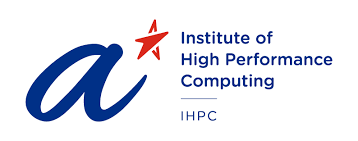
\includegraphics[height=1.5cm]{figures/ichpc.png}}\hspace*{20pt}
    \raisebox{20pt}[10pt][10pt]{
\includegraphics[height=4cm]{../logos/unimi_logo.pdf}}\hspace*{20pt}
    \raisebox{20pt}[10pt][10pt]{
\includegraphics[height=4cm]{../logos/tii_logo.png}}\hspace*{20pt}
    \raisebox{30pt}[10pt][10pt]{
\includegraphics[height=3cm]{figures/cqt.png}}
    % \includegraphics[height=1.3cm]{../_logos/erc_logo1.png}

    % \vfill\vspace*{230pt}
    % 
\includegraphics[height=1cm]{../_logos/unimi_logo.png}\hfill
    % 
\includegraphics[height=1cm]{../_logos/infn_logo.png}\\
    % \vspace*{5pt}
    % {
    %     \fontsize{3pt}{3.5pt}\selectfont
    %     \begin{center}
    %         This project has received funding from the European Union's Horizon
    %         2020 research and innovation programme under grant agreement No
    %         % 740006\quad \includegraphics[height=5pt]{../_logos/eu-flag.jpg}
    %     \end{center}
    % }
}
\setbeamercolor{background canvas}{bg=white}

\begin{document}

\maketitle

\setbeamertemplate{section in toc}[square]
\begin{frame}{Outline}
\tableofcontents
\end{frame}

\section{Basic elements of classical logic}
\begin{frame}{Binary code}
    A classical computer operates on string of zeros and ones, also known as binary code.
    \begin{multicols*}{2}
        \begin{figure}
            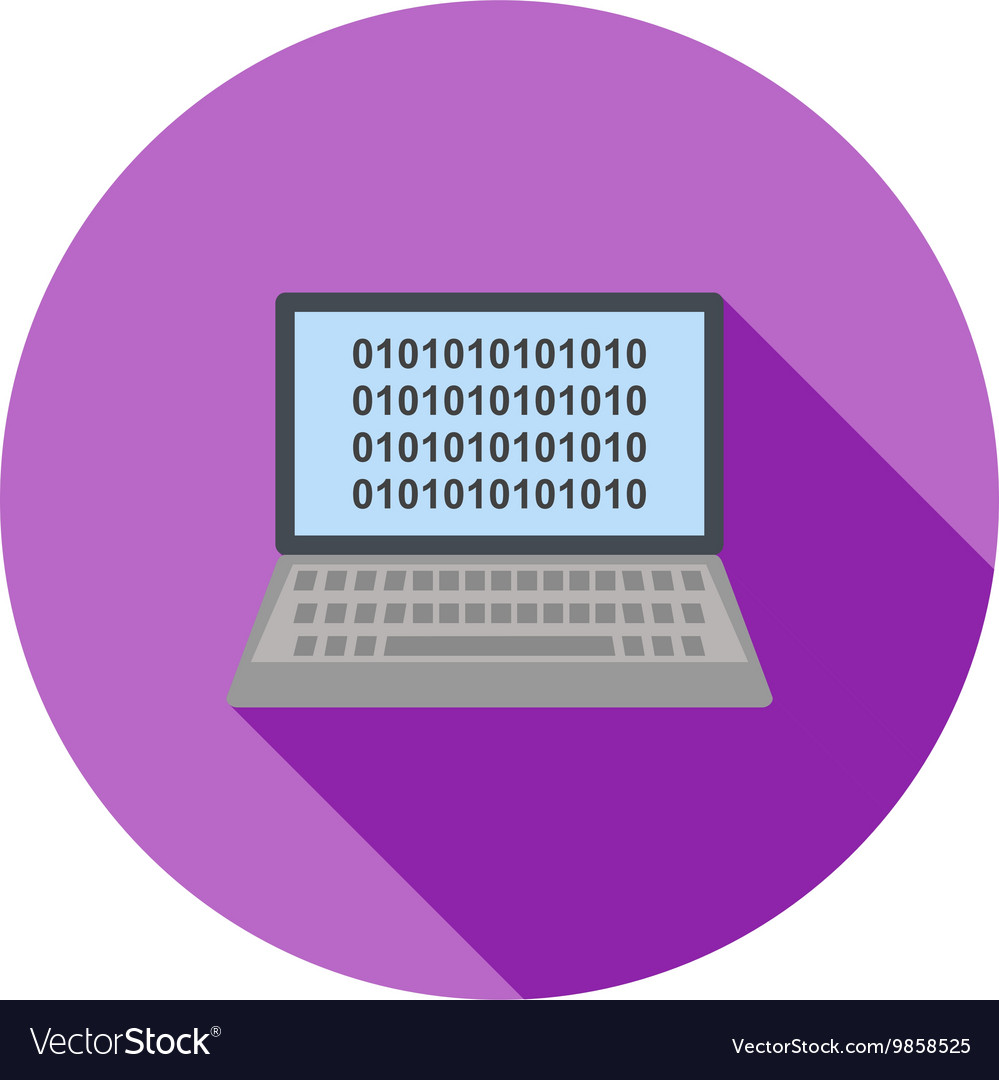
\includegraphics[width=0.5 \textwidth]{figures/binary_code.jpg}
        \end{figure}  

        \begin{figure}
            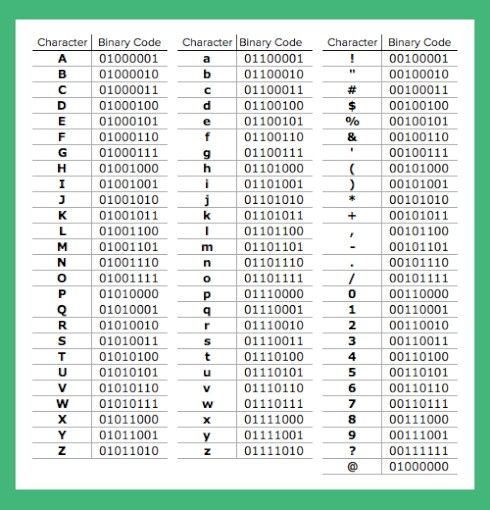
\includegraphics[width=0.5 \textwidth]{figures/binary.jpg}
        \end{figure}  
    \end{multicols*}
    
    
\end{frame}

\begin{frame}{Binary code}
    A binary string is composed by several binary variables, which are categorical
    variables which can take only one of two values (usually denoted by 0 and 1).
    \begin{tcolorbox}
        A \textbf{bit} is defined as the amount of information carried by a binary variable.
    \end{tcolorbox}
    

    We can represent the state of a bit using the following notation:

    $$ 0 \rightarrow \ket{0} $$
    $$ 1 \rightarrow \ket{1} $$

Therefore the state of 4 classical bits representing 1010 can be represented as 
$$ \ket{1} \ket{0} \ket{1} \ket{0} $$

It is also possible to associate with $\ket{0}$ and $\ket{1}$ two column vectors:

$$ \ket{0} \rightarrow \begin{pmatrix}
    1 \\ 
    0
\end{pmatrix}   \quad \text{and} \quad \ket{1} \rightarrow \begin{pmatrix}
    0 \\ 
    1
\end{pmatrix} $$
\end{frame}

\begin{frame}{Classical logical operations}
    We can change the value of a bit using logical opeartions.

    It can be shown that \textbf{any} logical or arithmetical operation can be
    obtained by the composition of three elementary logical operations:

    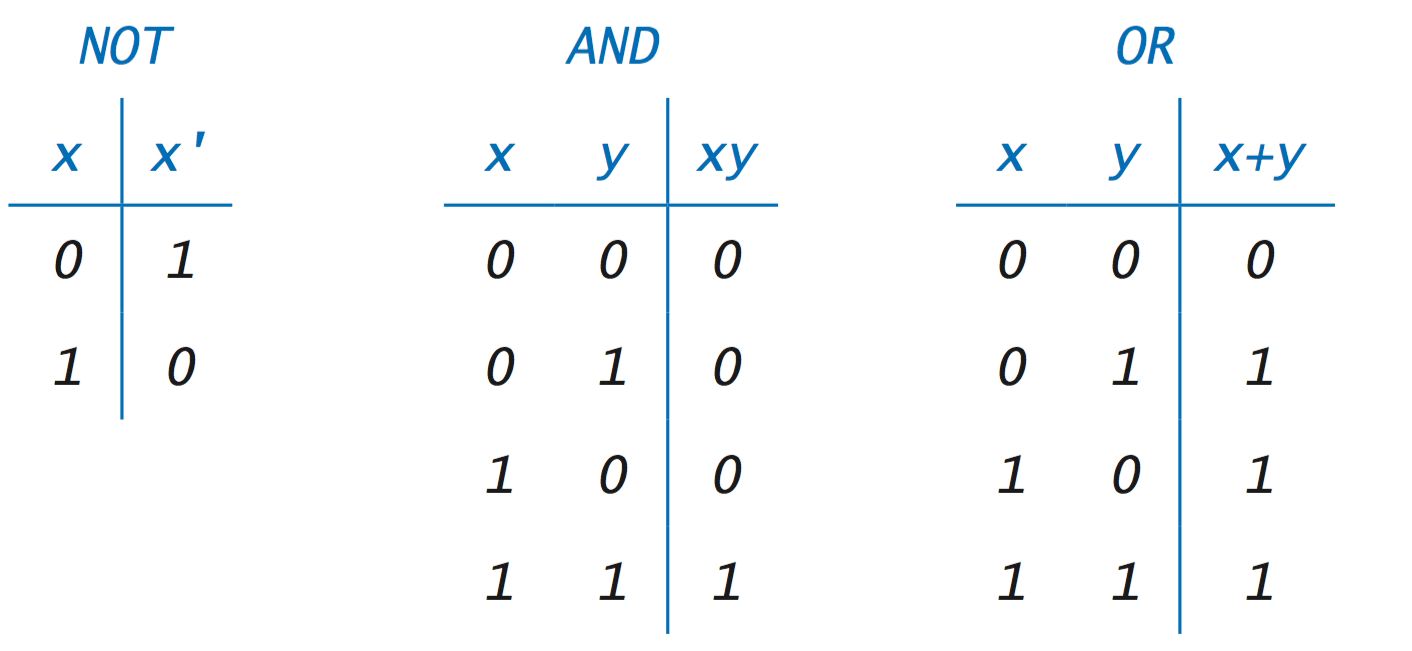
\includegraphics[width=\textwidth]{figures/truth-table.png}
    
\end{frame}

\begin{frame}{Reversible logical operations}
    In Quantum Computing we are mainly interested in reversible operation.

    \begin{tcolorbox}[title=Reversible operation]
       A logic function is \textbf{reversible} if each output arises from a unique input.
    \end{tcolorbox}

    What is the only nontrivial reversible operation that we can apply to a single bit?
    
    \pause

    The \textbf{NOT} operation, denoted by the symbol $\textbf{X}$ which flips the state of a bit

    $$ \textbf{X} : \ket{0} \rightarrow \ket{1} $$
    $$ \textbf{X} : \ket{1} \rightarrow \ket{0} $$

    Using the vector notation we can represent this gate as a matrix

    $$ \textbf{X} \rightarrow \begin{pmatrix}
        0 & 1 \\
        1 & 0
    \end{pmatrix}$$

    Not is reversible since if we apply $\textbf{X}$ a second time we go back to the
    original state
    $$ \textbf{X}^2 = \textbf{I} $$
\end{frame}

\begin{frame}{Two-bit reversible operations: SWAP}
    What about two-bit reversible operations?

    The most general reversible operation on two bits is any permutation of their four 
    possible states. We will show two gates $\textbf{SWAP}$ and $\textbf{CNOT}$.
    \vspace{0.5cm}

    \pause
    The \textbf{SWAP} gate, $\textbf{S}_{ij}$,  exchanges the states of the bit $i$ and $j$.
    For a two-bit system we get the following:
    $$ \textbf{S}_{10} \ket{x} \ket{y} = \ket{y} \ket{x}$$
    In particular we have:
    \begin{multicols*}{2}
        \begin{itemize}{}
            \item $\textbf{S}_{10} \ket{0} \ket{0} = \ket{0} \ket{0} $
            \item $\textbf{S}_{10} \ket{0} \ket{1} = \ket{1} \ket{0} $
            \item $\textbf{S}_{10} \ket{1} \ket{0} = \ket{0} \ket{1} $
            \item $\textbf{S}_{10} \ket{1} \ket{1} = \ket{1} \ket{1} $
        \end{itemize}
    \end{multicols*}
    which corresponds to the following matrix representation:
    $$\textbf{S}_{01} = \begin{pmatrix}
        1 & 0 & 0 & 0 \\
        0 & 0 & 1 & 0 \\
        0 & 1 & 0 & 0 \\
        0 & 0 & 0 & 1 \\
    \end{pmatrix} $$
\end{frame}

\begin{frame}{Two-bit reversible operations: CNOT}
    One of the most important reversible operation, especially for quantum computing,
    is the \emph{controlled-NOT} operator, $\textbf{C}_{ij}$, which implement the following
    operation:
    \begin{itemize}
        \item if $\ket{i} = \ket{0} \Rightarrow$ do nothing
        \item if $\ket{i} = \ket{1} \Rightarrow$ apply NOT operator to $\ket{j}$
    \end{itemize}
    which can be summarized in the following compact form

    \begin{multicols*}{2}
        \begin{itemize}
            \item $\textbf{C}_{01} \ket{x} \ket{y} = \ket{x} \ket{y \oplus x} $
            \item $\textbf{C}_{10} \ket{x} \ket{y} = \ket{x \oplus y} \ket{y} $
        \end{itemize}
        
    \end{multicols*}

    \begin{multicols*}{2}
        \begin{itemize}
    \item $\textbf{C}_{01} = \begin{pmatrix}
        1 & 0 & 0 & 0 \\
        0 & 1 & 0 & 0 \\
        0 & 0 & 0 & 1 \\
        0 & 0 & 1 & 0 \\
    \end{pmatrix} $

    \item $\textbf{C}_{10} = \begin{pmatrix}
        1 & 0 & 0 & 0 \\
        0 & 0 & 0 & 1 \\
        0 & 0 & 1 & 0 \\
        0 & 1 & 0 & 0 \\
    \end{pmatrix} $

\end{itemize}
        
\end{multicols*}

It is clear that the CNOT gate acts as a generalized XOR gate \footnote{
    The operator $\oplus$ corresponds to summing the two bits modulo 2. So for example we have
    $ (0 + 1) \text{mod} 2 = 1 \text{mod} 2 = 1 = 0 \ \textbf{XOR} \ 1.$
}.
    
\end{frame}

\begin{frame}{Manipulating operations on Classical bits}
    It is also instructive to introduce the operator $\textbf{N}$:
    $$ \textbf{N} \ket{x} = x \ket{x}$$
    which projects onto the state $\ket{1}$.


    And its complementary
    $$ \tilde{\textbf{N}} = \textbf{1} - \textbf{N}$$
    which projects onto the state $\ket{0}$.


    The corresponding matrices are
    $$ \textbf{N} \rightarrow \begin{pmatrix}
        0 & 0 \\
        0 & 1 
    \end{pmatrix} \quad \text{and} \quad
     \tilde{\textbf{N}} \rightarrow \begin{pmatrix}
        1 & 0 \\
        0 & 0 
    \end{pmatrix} $$

\end{frame}

\begin{frame}{Manipulating operations on Classical bits}
    We can also introduce the $\textbf{Z}$ which is defined as
    $$ \textbf{Z} = \tilde{\textbf{N}} - \textbf{N} = 
    \begin{pmatrix}
        1 & 0 \\
        0 & -1 \\
    \end{pmatrix}$$ 
    which anticommutes with $\textbf{X}$ since $ \textbf{X}\textbf{Z} = - \textbf{Z}
    \textbf{X}$.

    Finally we introduce the Hadamard transformation which is defined as 
    $$ \textbf{H} = \frac{1}{\sqrt{2}}( \textbf{X} + \textbf{Z}) \rightarrow 
    \frac{1}{\sqrt{2}}\begin{pmatrix}
        1 & 1 \\
        1 & -1 
    \end{pmatrix}$$ .
    From a classical point of view $\textbf{H}$ is meaningless since it transforms a single
    bit state into a linear combinations of states
 
    $$ \textbf{H} \ket{0} = \frac{\ket{0} + \ket{1}}{\sqrt{2}} \quad \text{and}
    \quad 
    \textbf{H} \ket{1} = \frac{\ket{0} - \ket{1}}{\sqrt{2}}
    $$

     
\end{frame}

    \section{Brief overview on Quantum Mechanics}

\begin{frame}{Postulates of quantum mechanics}
    The postulates of quantum mechanics are a list of prescription to summarize:
    \pause
    \begin{enumerate}
        \item how to describe the state of a physical system
        \pause
        \item how to describe the measurement performed on a physical system \pause
        \item how to describe the evolution of a physical system
    \end{enumerate}
    
\end{frame}

\begin{frame}{Postulate 1: State of a quantum system}
    Each physical system is associated with a complex Hilbert space $\mathcal{H}$. 
    A state is a normalized vector $\ket{\psi}$, which contains all the information about the system.
    Futhermore, in QM the superposition principle holds:
    \begin{tcolorbox}[title=Superposition principle]
       If $\ket{\psi}$ and $\ket{\phi}$ are possibile states of a quantum system a state of the form
       $$ \ket{\xi} = \alpha \ket{\psi} + \beta \ket{\phi}$$ such that $\bra{\xi} \ket{\xi} = 1$ is 
       an admissible state of the system, with $\alpha$ and $\beta \in \mathbb{C}$.
     \end{tcolorbox}

     For a composite system we have:
     $$ \ket{\Psi} = \ket{\psi}_1 \otimes \cdots \otimes \ket{\psi}_N \in \mathcal{H} $$
     where $\mathcal{H}$ is the tensor product of the Hilbert spaces associated with each system.
    \end{frame}
\begin{frame}{Postulate 2: Quantum measurement}
    Observable quantities are described by Hermitian operators $A = {A}^\dagger$,
    therefore the operator $A$ admits a spectral decomposition in terms of real eigenvalues $a_i$,
    which are the possible values of the observable.

    The probability of obtaining the outcome $a_i$ from the measurement of $A$ in a given state
    $\psi$ is equal to

    $$ p(a_i) = | \bra{u_i} \ket{\psi}|^2 $$

    The overall expectation value of the observable $A$ is computed as

    $$ \expval{A} = \expval{A}{\psi} $$

    \begin{tcolorbox}
        If we measure the outcome $a_i$ the state of the system collapse to the correspoding eigeinvector
        of the observable $A$, such that:
        $$ A \ket{\alpha_i} = a_i \ket{\alpha_i} \quad \Rightarrow \ket{\psi} \rightarrow \ket{\alpha_i}$$
    \end{tcolorbox}

\end{frame}

\begin{frame}{Postulate 3: Dynamics of a quantum system}
    The dynamical evolution of a physical system  from an 
    initial time $t_0$ to a time $t \ge t_0$ is described by a 
    unitary operator $\textbf{U}(t, t_0)$

    $$\ket{\psi_t} = \textbf{U}(t, t_0) \ket{\psi_0}$$ \ .

    $\textbf{U}(t, t_0)$ is linked to the \emph{Hamiltonian} of the quantum system through the
    Schr\"{o}dinger equation

    $$ i \hbar \frac{\partial}{\partial t} \ket{\psi_t} = H \ket{\psi_t}$$

    where $H$ is the Hamiltonian of the system.

    For example, if the Hamiltonian is time independent, after solving the 
    Schr\"{o}dinger equation we find the following solution for $\textbf{U}(t, t_0)$:

    $$ \textbf{U}(t, t_0) = \exp(- i H (t -t_0))$$


    
\end{frame}

\section{Quantum Computing}

\begin{frame}{What is a Qubit?}
    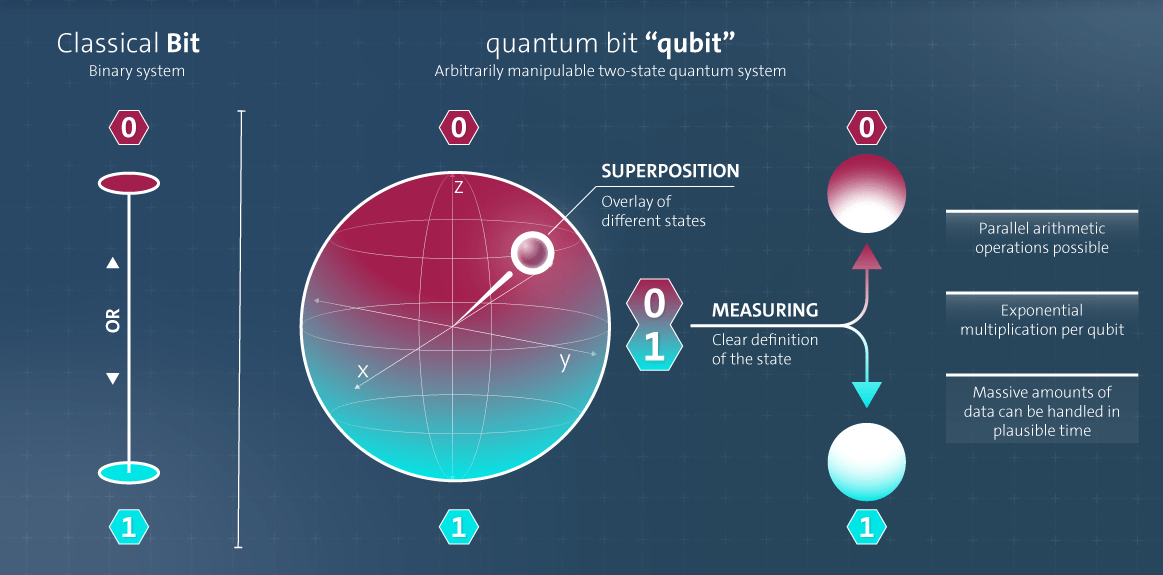
\includegraphics[width=\textwidth]{figures/qubits.png}
\end{frame}

\begin{frame}{What is a Qubit?}
    A state $\psi$ associated with a qubit is a generic two-level
    quantum system:

    $$ \ket{\psi} = \alpha \ket{0} + \beta \ket{1} \rightarrow 
    \begin{pmatrix}
        \alpha \\ 
        \beta
    \end{pmatrix}$$

    where $\alpha$ and $\beta$  are two complex numbers constrained
    by the requirement that $\ket{\psi}$, like 
    $\ket{0}$ and $\ket{1}$ should be a unit vector
    in the complex vector space. 
    
    This means that the 
    following normalization must hold
    
    $$|\alpha|^2 + |\beta|^2 = 1$$

    We can see that contrary to the classical case a qubit is associated
    with multiple states, and the most general expression is a superposition
    of the classical states $\ket{0}$ and $\ket{1}$.

\end{frame}

\begin{frame}{Bloch sphere}
    Since $|\alpha|^2 + |\beta|^2 = 1$ we can parametrize the amplitudes
    of the qubit state in the following way:

    $$ \alpha = \cos \frac{\theta}{2} \quad \text{and} \quad \beta = e^{i \phi} \sin \frac{\theta}{2}$$ 
    
    \begin{columns}
        \begin{column}{0.5 \textwidth}
            \vspace{1cm}

            We can associate with the qubit the following real numbers:

    $$ r_x = \sin \theta \cos \phi \, \quad r_y = \sin \theta \sin \phi \, \quad r_z = \cos \theta  $$
    which can be seen as the components of a 3-dimensional vector

    $$ \textbf{r} = 
    \begin{pmatrix}
        r_x \\ r_y \\ r_z
    \end{pmatrix} = 
    \begin{pmatrix}
        \sin \theta \cos \phi \\
        \sin \theta \sin \phi \\
        \cos \theta
    \end{pmatrix} 
    $$
        \end{column}

    \begin{column}{0.4 \textwidth}
        \begin{figure}
            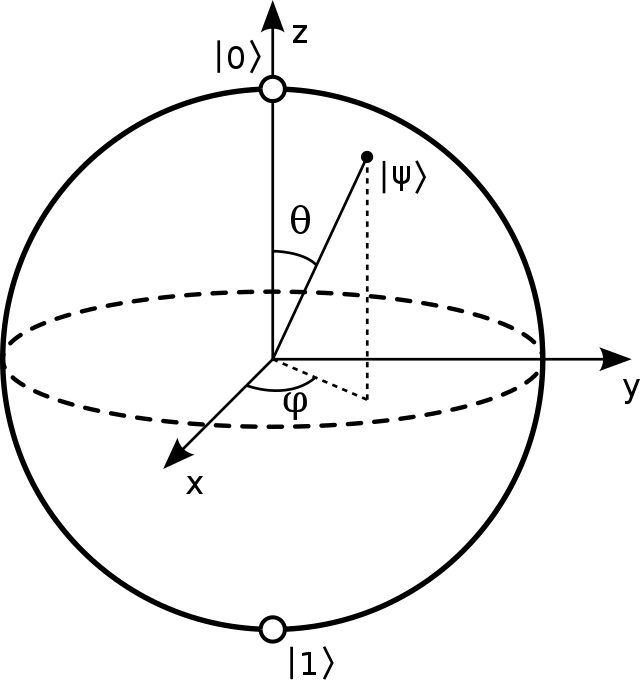
\includegraphics[width = \textwidth]{figures/Bloch_sphere.png}
        \end{figure}
        
    \end{column}
    \end{columns}
    
\end{frame}

\begin{frame}{Multiple qubit states}
    Just as the general state of a single qubit is 
    any normalized superposition of two possible classical state, the general state that the nature
    allows us to associate with two qubits is any normalized superposition of
    the four orthogonal classical states

    $$ \ket{\Psi} = \alpha_{00} \ket{00}
                  + \alpha_{01} \ket{01}
                  + \alpha_{10} \ket{10}
                  + \alpha_{11} \ket{11}$$
    with the normalization condition 
    $ |\alpha_{00}|^2 + |\alpha_{01}|^2 + 
    |\alpha_{10}|^2 + |\alpha_{11}|^2 = 1$

    For a $n$ qubit system we have the following expression

    $$ \Psi = \sum_{x = 0}^{2^n - 1} \alpha_x \ket{x}_n \quad 
    \text{with} \quad \sum_{x = 0}^{2^n - 1} |\alpha_x|^2 = 1$$

    We observe that the we are summing over $2^n$ values since
    there are $2^n$ classical states that one could obtain by looking
    at all the possible tensor products.

\end{frame}

\begin{frame}{Reversible operations on qubits}
    We have already observed that the only nontrivial reversible operation
    that can performed on a classical bit is the NOT operation \textbf{X}.
    
    In QM we can modify a state by applying an \emph{unitary} transformation, see postulate 3,
    \textbf{u}, which by definition satisfy the following condition
    $$ \textbf{u} \textbf{u}^\dagger = \textbf{u}^\dagger \textbf{u} = 1  $$

    Since any unitary transformation has a unitary inverse, such actions of a quantum
    computer on a qubit are fully reversible.

    The previous equation holds for a generic system with $n$ qubits, in particular we
    have that in order to modify a $n$ qubit system we can act with a $2^n \times 2^n$ unitary matrix.
\end{frame}


\begin{frame}{Quantum logic gates}
    It is possible to represent schematically the action of a unitary transformation $\textbf{u}$ on a
    qubit state $\ket{\psi}$ using the following picture
    $$
    \begin{quantikz}
        \lstick{$\ket{\psi}$} & \qw & \gate{\textbf{u}} &\qw
        & \rstick{$\textbf{u} \ket{\psi} = \ket{\psi '}$} \qw
        \end{quantikz}
        $$
        which in quantum computing is called a \textbf{quantum circuit}.

    What happens if we apply more than one gate?
    
    Suppose that we apply two unitary transformations $\textbf{u}_1$ and $\textbf{u}_2$ on the state $\ket{\psi}$

    $$ \ket{\psi'} = \textbf{u}_1 \textbf{u}_2 \ket{\psi}$$
    We can again represent these transformations using a quantum circuit.
    $$
    \begin{quantikz}
        \lstick{$\ket{\psi}$} & \qw & \gate{\textbf{u}_2} & \qw &  \gate{\textbf{u}_1} &\qw
        & \rstick{$\ket{\psi '}$} \qw
        \end{quantikz}$$ 

    \begin{tcolorbox}[title=Observation]
        The sequence of symbols is reverse from the sequence in which they appear in the mathematical expression!
    \end{tcolorbox}
    
    
\end{frame}

\begin{frame}{One qubit gates}
    Here are the most common used one qubit gates.

    \begin{figure}
        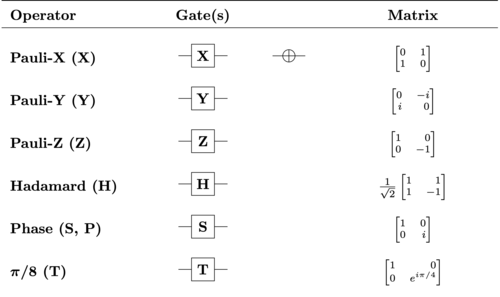
\includegraphics[width=\textwidth]{figures/Quantum_Logic_Gates_1.png}
    \end{figure}
    Lets have a closer look to some of them.
\end{frame}

\begin{frame}{$\textbf{X}$ and $\textbf{Z}$ gates}

    \begin{columns}
        \begin{column}{0.5 \textwidth}
            \begin{tcolorbox}[title=$\textbf{X}$ gate]
                The $\textbf{X}$ gate acts as the classical NOT gate, it is represented by  $\sigma_x$ 

                $$ \sigma_x = \begin{pmatrix}
                    0 &  1 \\
                    1 & 0
                \end{pmatrix}$$
                therefore we get 
                $$
                \begin{quantikz}
                    \lstick{$\ket{0}$} & \qw & \gate{\textbf{X}} &\qw
                    & \rstick{$\ket{1}$} \qw
                    \end{quantikz}
                    $$

                    $$
                    \begin{quantikz}
                        \lstick{$\ket{1}$} & \qw & \gate{\textbf{X}} &\qw
                        & \rstick{$\ket{0}$} \qw
                        \end{quantikz}
                        $$

             \end{tcolorbox}
        \end{column}

        \begin{column}{0.5 \textwidth}
            \begin{tcolorbox}[title=$\textbf{Z}$ gate]
                The $\textbf{Z}$ gate flips the sign of $\ket{1}$, it is represented by the $\sigma_z$

                $$ \sigma_z = \begin{pmatrix}
                    1 &  0 \\
                    0 & -1
                \end{pmatrix}$$
                therefore we get 
                $$
                \begin{quantikz}
                    \lstick{$\ket{0}$} & \qw & \gate{\textbf{Z}} &\qw
                    & \rstick{$\ket{0}$} \qw
                    \end{quantikz}
                    $$

                    $$
                    \begin{quantikz}
                        \lstick{$\ket{1}$} & \qw & \gate{\textbf{Z}} &\qw
                        & \rstick{$- \ket{1}$} \qw
                        \end{quantikz}
                        $$

             \end{tcolorbox}
        \end{column}
    \end{columns}

    
\end{frame}

\begin{frame}{Hadamard gate}
    The Hadamard gate $\textbf{H}$ is represented by the following matrix 
    $$ \textbf{H} \rightarrow \frac{1}{\sqrt{2}}
    \begin{pmatrix}
       1 & 1 \\
       1 & -1  
    \end{pmatrix}
    $$
    It is extremely important in quantum computing since it can create a superposition of states

    $$
    \begin{quantikz}
        \lstick{$\ket{0}$} & \qw & \gate{\textbf{H}} &\qw
        & \rstick{$\frac{\ket{0} + \ket{1}}{\sqrt{2}}$} \qw
        \end{quantikz}
        $$

        $$
    \begin{quantikz}
        \lstick{$\ket{1}$} & \qw & \gate{\textbf{H}} &\qw
        & \rstick{$\frac{\ket{0} - \ket{1}}{\sqrt{2}}$} \qw
        \end{quantikz}
        $$
\end{frame}

\begin{frame}{Two-qubits gate}
    \begin{figure}
        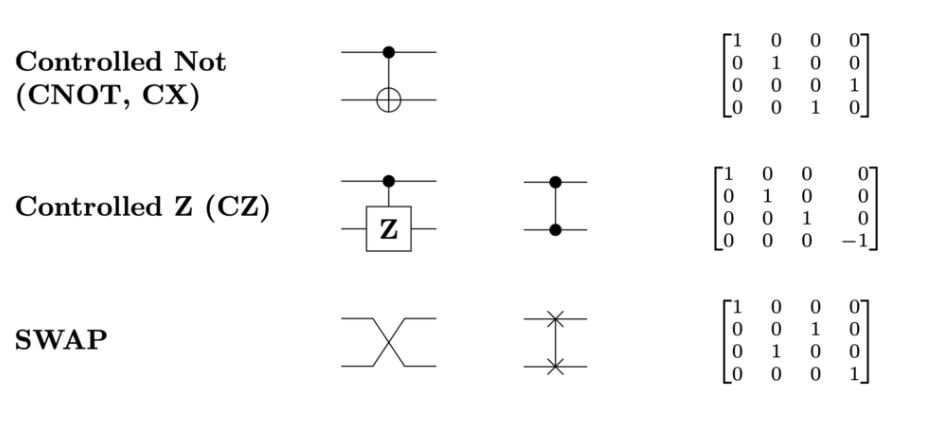
\includegraphics[width = \textwidth]{figures/two_qubits_gates.png}
    \end{figure}
\end{frame}   
\begin{frame}{\textbf{CNOT} gate}
    The prototypical multi-qubit quantum logic gate is the controlled-$\textbf{NOT}$ or $\textbf{CNOT}$ gate.
This gate has two input qubits, known as the \emph{control} qubit and the \emph{target} qubit.


    \begin{figure}
        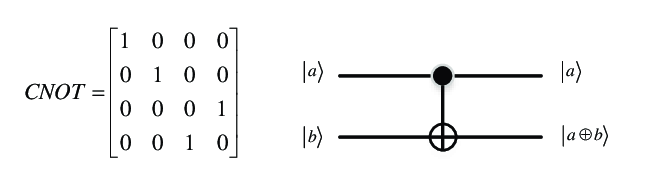
\includegraphics[width=0.5 \textwidth]{figures/cnot.png}
    \end{figure}

    In the case where the first qubit is the control qubit we get the matrix $\textbf{C}_{01}$
    if we swap target and control qubit we get $\textbf{C}_{10}$.
    
    We can observe that $\textbf{C}_{01}$ can be rewritten in the following way:

    $$ \textbf{C}_{01} = \begin{pmatrix}
        \mathbf{1} & 0 \\
        0 & \sigma_x
    \end{pmatrix} = \textbf{CNOT}$$.

   Can we generalize this expression for a generic unitary matrix $\textbf{U}$?
\end{frame}

\begin{frame}{Generic controlled gate}
    The conditional application of a unitary transformation $\textbf{U}$ to a qubit namely 
    $$ c\textbf{U} \ket{x} \ket{y} = \mathbf{1} \otimes \textbf{U}_x \ket{x} \ket{y}$$
    Can be represented through the following 4x4 matrix:
    $$ c\textbf{U} \rightarrow \begin{pmatrix}
        \textbf{1} & 0 \\
        0 & \textbf{U}
    \end{pmatrix}$$
    under the assumption the first qubit is the control qubit.

    As an example the $\textbf{CZ}$ can be represented as follows:

    $$ \textbf{CZ} \rightarrow \begin{pmatrix}
        1 & 0 & 0 & 0 \\
        0 & 1 & 0 & 0 \\
        0 & 0 & 1 & 0 \\
        0 & 0 & 0 & -1 \\
    \end{pmatrix} = 
    \begin{pmatrix}
        \textbf{1} & 0 \\
        0 &  \sigma_z
    \end{pmatrix}
        $$    
\end{frame}

\begin{frame}{Gates with more than 2 qubits?}
    What about gates with more that 2 qubits?
    As an example we present the $\textbf{TOFFOLI}$ gate, which is represented by the unitary operator $\textbf{T}$.

    The $\textbf{T}$ gate acts on the computational basis as follows:

    $$ \textbf{T} \ket{x} \ket{y} \ket{z} = \ket{x} \ket{y} \ket{z \oplus xy}$$

    It is particulary useful in quantum computing since it enables us to perform an $\textbf{AND}$ gate of two bits
    and the $\textbf{NOT}$ gate, in fact

    $$ \textbf{AND} \rightarrow \textbf{T} \ket{x} \ket{y} \ket{0} =  \ket{x} \ket{y} \ket{xy} \equiv \ket{x} \ket{y} \ket{x \wedge y}$$
    $$  \textbf{NOT} \rightarrow \textbf{T} \ket{1} \ket{1} \ket{x} =  \ket{1} \ket{1} \ket{x \oplus 1} \equiv \ket{1} \ket{1} \ket{\bar{x}}$$

    Since all logical and mathematical operations can be built out of AND and NOT, we have shown that using the TOFFOLI gate
    we can reproduce all these operations on a quantum computer, i.e. reversibly.
\end{frame}

\begin{frame}{Measurements}
    % To extract the information contained into a set of classical bits it is sufficient to \emph{look}.
    % In particular, the act of acquiring information form classicl bits is not disruptive.

    For a quantum system, in order to extract information, we need to make a \textbf{measurement}, which corresponds
    to perfoming a certain opeartion on each qubit, the outcome of which is either 0 and 1.\footnote{
        The observable that we are measuring in this case is the $\textbf{Z}$ operator.
    }

    Futhermore, we know from postulate 2, that the state determines only the \emph{probability} of the
    possible outcomes which is given the by squared magnitude of the amplitudes.

    If we have the following state:

    $$ \ket{\psi} = \sum_{x = 0}^{2^n - 1} \alpha_x \ket{x} $$

    the probabiility of measuring a specific state $\ket{y}$ is given by

    $$ p (y) = |\bra{y} \ket{\psi} |^2 = |\alpha_y|^2 \ .$$

    It is now clear that measuring a qubit requires a \emph{statistical} approach, this is why we talk 
    about expected values of the observables.

\end{frame}

\begin{frame}{Irreverisbility of measurements}
    Contrary to all the other operations, the measurement is an \textbf{irreversible} operation.

    $$
    \begin{quantikz}
        \lstick{$\ket{\psi}$} & \qw & \gate{\textbf{u}} &\qw
        & \meter{} & \qw \rstick{$\ket{0}$} \qw
        \end{quantikz}
        $$
    In particular, this operation is irreversible since we are losing information about the system.
    
    \emph{What information exactly?}

    \pause

    After we measure a quantum system, the state collapse to the eigenstate associated with the measurement
    outcome. Therefore, we no longer have access to the information available in the amplitudes of the 
    state $\ket{\psi}$.
    
\end{frame}

\begin{frame}{State preparation}
    Supppose that we want to prepare our quantum system in a specific state, how can we produce that
    particular state? 

    \pause 
    We can do it  by \textbf{measuring} the system.
    \pause

    This initial action of the measurement gate is called \textbf{state preparation}, since after this first
    step we have created a definite state.

    Is there another way?

    \pause

    For some particular physical realizations of qubits, yes. 

    For example, if each qubit is an atom, by cooling the system to an approriate low temperature
    we can produce the state $\ket{0}_n$


\end{frame}

\section{Applications}

\begin{frame}{CNOT and No-cloning theorem}
    One of the most interesting result in QM is the no-cloning theorem which state the following:

   \begin{tcolorbox}[title=No-cloning theorem]
    Assume we have a unitary operator $U_{cl}$ and two quantum states $\ket{\phi}$ and $\ket{\psi}$ which
    $U_{cl}$ copies,

    $$ U_{cl} \ket{\phi} \otimes \ket{0} = \ket{\phi} \otimes \ket{\phi}$$
    $$ U_{cl} \ket{\psi} \otimes \ket{0} = \ket{\psi} \otimes \ket{\psi}$$

    then $\bra{\phi} \ket{\psi}$ is 0 or 1.
   \end{tcolorbox}

   This theorem is telling us that we cannot create an identical copy of an arbitrary unknown quantum state.

   It is possible to verify this theorem using quantum computing, in particular the $\textbf{CNOT}$ gate.
\end{frame}

\begin{frame}{CNOT and No-cloning theorem}
    Copying a classical bit is fairly easy using a $\textbf{XOR}$ or $\textbf{CNOT}$ gate 

    \begin{figure}
        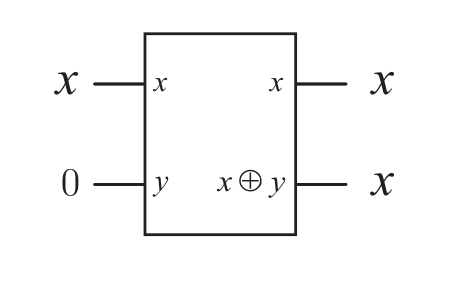
\includegraphics[width=0.5 \textwidth]{figures/copy_classical.png}
    \end{figure}
    Lets try to do the same thing with a quantum circuit.
\end{frame}

\begin{frame}{CNOT and No-cloning theorem}
    Suppose that we try to copy a qubit in the unknown state $\ket{\psi} = a \ket{0} + b \ket{1}$
    in the same manner.

    $$  \ket{\psi} \ket{0} = ( a \ket{0} + b \ket{1} ) \ket{0} = a \ket{00} + b \ket{10}$$

    If we apply the $\textbf{CNOT}$ gate we get the following:

    $$ \textbf{CNOT} a \ket{00} + b \ket{10} = a \ket{00} + b \ket{11}$$ 

    Have we actually copied the state $\ket{\psi}$?

    Lets compute the state $\ket{\psi} \ket{\psi}$:

    $$ \ket{\psi} \ket{\psi} = a^2 \ket{00} + ab \ket{01} + ab \ket{10} + b^2 \ket{11}$$

    Unless $ab = 0$, i.e. the state are orthogonal, we are not able to copy the state $\psi$ which 
    is exactly the statement of the theorem.
\end{frame}


\begin{frame}{Entanglement and Bell states}
    A key ingredient in quantum computing is the possibility to create entanglement. But what is entanglement?

    If for a multi-qubit system we are able to write the state as a tensor product of single-qubit states
    
    $$ \ket{\Psi}_N = \ket{\psi}_1 \otimes \cdots \otimes \ket{\psi}_N $$

    we say that the state $\ket{\Psi}$ is \emph{factorized} or \emph{separable}.

    \begin{tcolorbox}[title=Entagled state]
        A state which is \textbf{not} separable is called \emph{entangled}.
    \end{tcolorbox}
        For example the following state is entangled:

        $$ \ket{\Psi} = \frac{\ket{0}\ket{0} + \ket{1}\ket{1}}{\sqrt{2}}$$
    
\end{frame}

\begin{frame}{Bell states}
    We can recreate easily the entagled state of the previous slide using the following circuit.
    \begin{figure}
        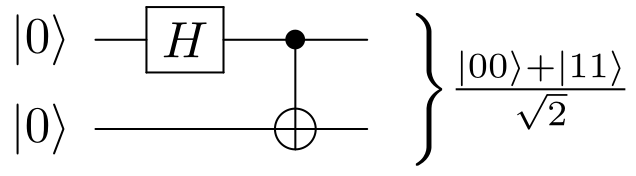
\includegraphics[width= 0.5 \textwidth]{figures/bell_circuit.png}
    \end{figure}
    This state is one of the four \emph{Bell states} or \emph{EPR state}, which are maximally entangled two qubits state.
    The other ones can be generated by acting with the same circuit on different initial state:

    \begin{multicols*}{2}
        \begin{itemize}
            \item $\ket{00} \rightarrow \ket{\beta_{00}} = \frac{\ket{0}\ket{0} + \ket{1}\ket{1}}{\sqrt{2}}$
            \item $\ket{01} \rightarrow \ket{\beta_{01}} = \frac{\ket{0}\ket{1} + \ket{1}\ket{0}}{\sqrt{2}}$
            \item $\ket{10} \rightarrow \ket{\beta_{10}} = \frac{\ket{0}\ket{0} - \ket{1}\ket{1}}{\sqrt{2}}$
            \item $\ket{11} \rightarrow \ket{\beta_{11}} = \frac{\ket{0}\ket{1} - \ket{1}\ket{0}}{\sqrt{2}}$
        \end{itemize}
        
    \end{multicols*}

\end{frame}
\section{Introduction to quantum algorithms}

\begin{frame}{The general computational process}
    \begin{itemize}
        \item A suitable programmed quantum computer should actor on a number $x$ to produce another number
        $f(x)$ for some specified function $f$.
        \item Since we expect $f$ to be not reversible we shall need at least $n+m$ qubits, assuming x is a
        $n$ bit integers and $f(x)$ an $m$-bit integer. Usually we call \emph{input register} the set of qubits
        that represent $x$ and \emph{output register} the set of qubits that represent $f(x)$.
        \item To perform the calculation of $f(x)$ we apply a suitable tranformation $\textbf{U}_f$ to our set of
        $n+m$ qubits:

        $$ \textbf{U}_f (\ket{x}_n \ket{y}_m) = \ket{x}_n \ket{y \oplus f(x)}_m  $$

        where $\oplus$ indicates the modulo-2 bitwise addiction or the XOR .

        If the initial value of the output register is $y=0$ we can obtain the actual value of $f(x)$

        $$ \textbf{U}_f (\ket{x}_n \ket{0}_m) = \ket{x}_n \ket{f(x)}_m  $$

    \end{itemize}

\end{frame}

\begin{frame}{The general computational process}
    We can also observe that $\textbf{U}_f$ is clearly invertible, as expected

    $$ \textbf{U}_f \textbf{U}_f (\ket{x} \ket{y}) = \textbf{U}_f \ket{x} \ket{y \oplus f(x)}
    = \ket{x} \ket{y} $$

    since $z \oplus z = 0$ for any $z$.


\end{frame}

\begin{frame}{Useful identities}
    Before looking at some quantum algorithms it is useful to learn a few identities.

    For a single qubit we write the action of the Hadamard gate in the following form:

    $$\textbf{H} \ket{x} = \frac{\ket{0}+ (-)^x \ket{1}}{\sqrt{2}} = 
    \frac{1}{\sqrt{2}} \sum_{z=0,1} (-)^{xz} \ket{z} $$

    For a $n$ qubits system we get

    $$ \textbf{H}^{\otimes n} \ket{x}_n = 
    \frac{\ket{0}+ (-)^{x_{n-1}} \ket{1}}{\sqrt{2}} \otimes \cdots \otimes 
     \frac{\ket{0}+ (-)^{x_0} \ket{1}}{\sqrt{2}} =
     \frac{1}{2^{n/2}} \sum_{z=0}^{2^n - 1} (-)^{xz} \ket{z}
      $$

    Finally if $f(x) \in \{ 0, 1 \}$ then we have

    $$ \textbf{U}_f (\textbf{I} \otimes \textbf{H})  \ket{x}\ket{1} 
    = \ket{x} \frac{\ket{f(x)} - \ket{1 \oplus f(x)}}{\sqrt{2}} = (-)^{f(x)} \ket{x} \frac{\ket{0} - \ket{1}}{\sqrt{2}}
    $$
\end{frame}

\begin{frame}{Deutsch algorithm}
    As a first example lets have a look at the Deutsch problem
    \begin{tcolorbox}[title=Deutsch problem]
        Given a function $f : \{0, 1 \} \rightarrow  \{0, 1 \}$ we want to know whether if $f(0) = f(1)$.
    \end{tcolorbox}

    From a classical point of view of how many times do we need to evaluate $f(x)$? 
    \pause 
    Correct answer: 2

    We are going to show that a quantum algorithm can tell us the answer using just one evaluation
     of the function $f$ using the following circuit:

     \begin{figure}
        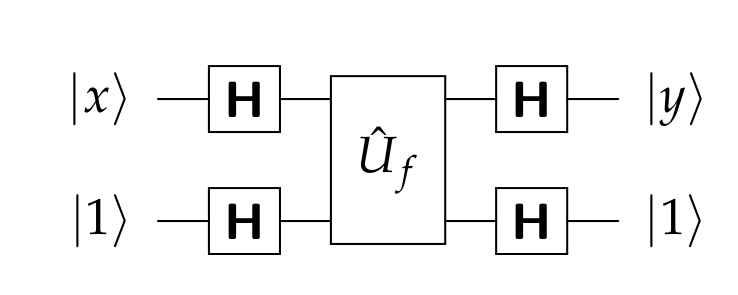
\includegraphics[width = 0.5 \textwidth]{figures/deutsch.png}
     \end{figure}


\end{frame}

\begin{frame}{Deutsch algorithm}
    Lets apply the quantum circuit of the previous slide step by step:

    \begin{enumerate}
        \item Apply $\textbf{H}$ to both qubits in the initial state
        $$ \textbf{H} \otimes \textbf{H} \ket{x} \ket{1} =
        \sum_z \frac{(-)^{xz}}{\sqrt{2}} \ket{z} \frac{\ket{0} - \ket{1}}{\sqrt{2}}
        $$
        where we used one the identities from the previous slides.
        \item Apply $\textbf{U}_f$
        $$ \textbf{U}_f \sum_z \frac{(-)^{xz}}{\sqrt{2}} \ket{z} \frac{\ket{0} - \ket{1}}{\sqrt{2}} 
        = \sum_z \frac{(-)^{xz + f(z)}}{\sqrt{2}} \ket{z} \frac{\ket{0} - \ket{1}}{\sqrt{2}}  $$
        \item Apply again the Hadamard transformations
        $$ ( \textbf{H} \otimes \textbf{H}) \textbf{U}_f  ( \textbf{H} \otimes \textbf{H}) \ket{x} \ket{1}
        = \sum_{s = 0,1} c_f(x, s) \ket{s} \ket{1} $$
        where we have introduce the coefficients:
         
        $$ c_f(x, s) = \frac{1}{2} (-)^{f(0)} \big[ 1 + (-)^{x+s} (-)^{f(1) - f(0)}\big] $$
    \end{enumerate}
\end{frame}

\begin{frame}{Deutsch algorithm}
    It is straightforward to verify that
    \begin{itemize}
        \item if $f(1) = f(0) \Rightarrow |c_f(x,x)|^2 = 1$ and $|c_f(x,\bar{x})|^2 = 0$
        \item if $f(1) \neq f(0) \Rightarrow |c_f(x,x)|^2 = 0$ and $|c_f(x,\bar{x})|^2 = 1$
    \end{itemize}
    Therefore, if a measurement on the input register gives result $\ket{x}$ we can conclude that $f(0) = f(1)$
    if it leads to $\ket{\bar{x}}$ we have $f(1) \neq f(0)$.

    All of this only with a single query of $\textbf{U}_f$!

\end{frame}

\begin{frame}{Quantum algorithms}

    The Deutsch algorithm is just one of many quantum algorithms that are currently known.

\begin{multicols*}{3}
    \begin{tcolorbox}[title=Gate Circuits]
        \begin{itemize}
            \item Search (Grover)
            \item QFT (Shor)
            \item Deutsch
            \item $\dots$   
            \end{itemize}
     \end{tcolorbox}

\begin{tcolorbox}[title=Variational]
    \begin{itemize}
        \item Eigeinsolvers
        \item Autoencoders
        \item Classifiers
        \item $\dots$   
        \end{itemize}
 \end{tcolorbox}

 \begin{tcolorbox}[title=Annealing]
    \begin{itemize}
        \item Direct annealing
        \item Adiabatic evolution
        \item QAOA
        \item $\dots$   
        \end{itemize}
 \end{tcolorbox}

\end{multicols*}
    
\end{frame}

\section{Towards Quantum Machine Learning}

\begin{frame}{Variational Quantum Circuits}
    Getting inspiration from \textbf{AI}:
    \begin{itemize}
        \item Supervised learning $\Rightarrow$ Regression and classification
        \item Unsupervised learning $\Rightarrow$ Generative models, autoencoders
        \item Reinforcement learning $\Rightarrow$ Quantum RL / Q-learning
    \end{itemize}

    \vspace{2cm}

    Define new parametric model architectures for quantum hardware:


    \centering
    { \color{blue} $\Rightarrow$ Variational Quantum Circuits / Quantum Machine Learning}
\end{frame}

\begin{frame}{Rational for Variational Quantum Circuits}

    \textbf{Rational}:

    Deliver a variational quantum state that can explore a large Hilbert space

    \begin{figure}
        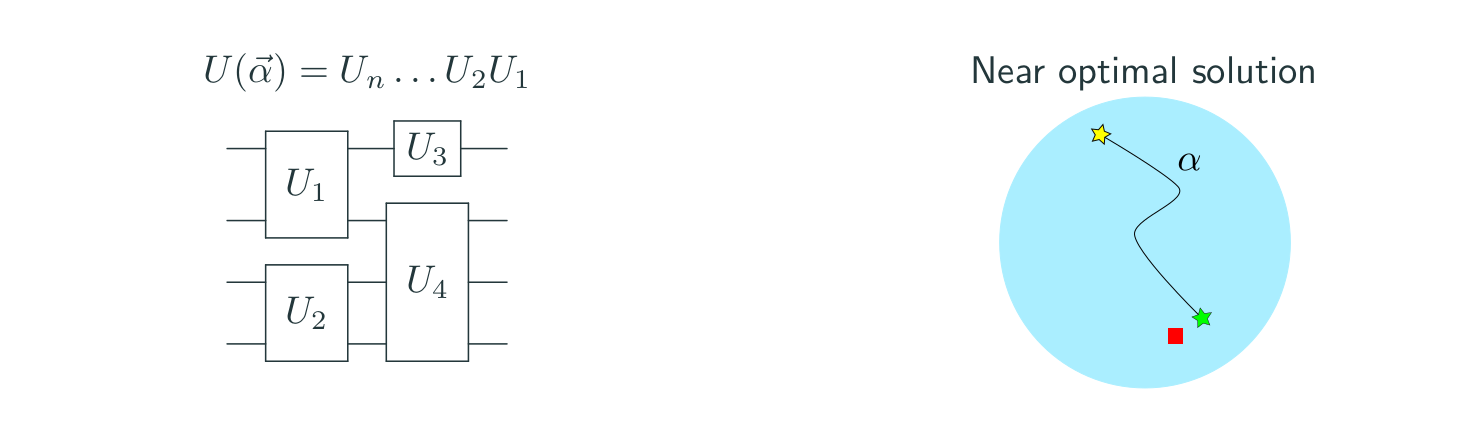
\includegraphics[width=\textwidth]{figures/variational.png}
    \end{figure}
    
    \textbf{Idea}:
    Quantum Computer is a machine that generates variational states.

    $\Rightarrow$ \textbf{Variational Quantum Computer}
\end{frame}

\begin{frame}{Solovay-Kitaev Theorem}
    \begin{columns}
        \begin{column}{0.5 \textwidth}
            Let $\{U_i \}$ be a dense set of unitaries.

            Define a circuit approximation to $V$:

            $$ |U_k \ldots -V| < \delta $$
            
            Scaling to best approximation

            $$ k \sim \mathcal{O}\Big( \log^c \frac{1}{\delta}\Big)$$

            where $c < 4$.
        \end{column}

        \begin{column}{0.5 \textwidth}

            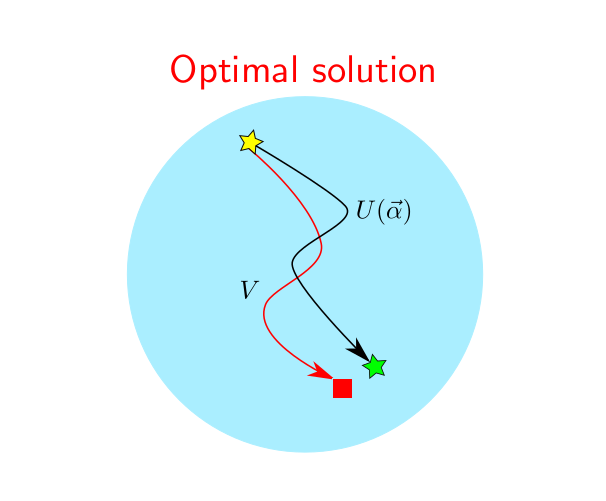
\includegraphics[width=\textwidth]{figures/optimal.png}
            
        \end{column}
    \end{columns}

    $\Rightarrow$ The approximation is \textbf{efficient} and requires a \textbf{finite} number of gates
    
\end{frame}
% \begin{frame}{Entropy of entanglement}
%    We can measure the entropy of a bipartite system using the Von Neumann entropy which is defined as 
%    $$ S[\rho] = - \text{Tr} [ \rho \log_2 \rho] $$

%    where $\rho$ 
% \end{frame}
\section{Quantum Technology}

\begin{frame}{Quantum technologies}
    \begin{figure}
        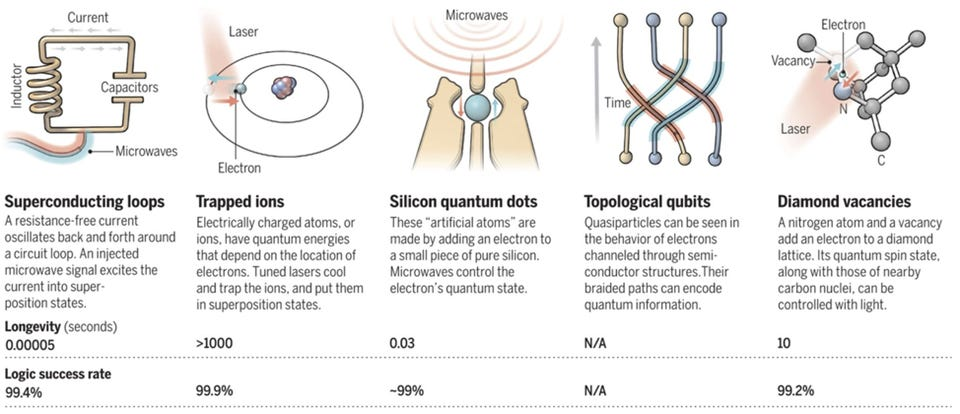
\includegraphics[width=\textwidth]{figures/q_technologies.jpg}
    \end{figure}
    
\end{frame}

\begin{frame}{Physical implementation}
    \begin{figure}
        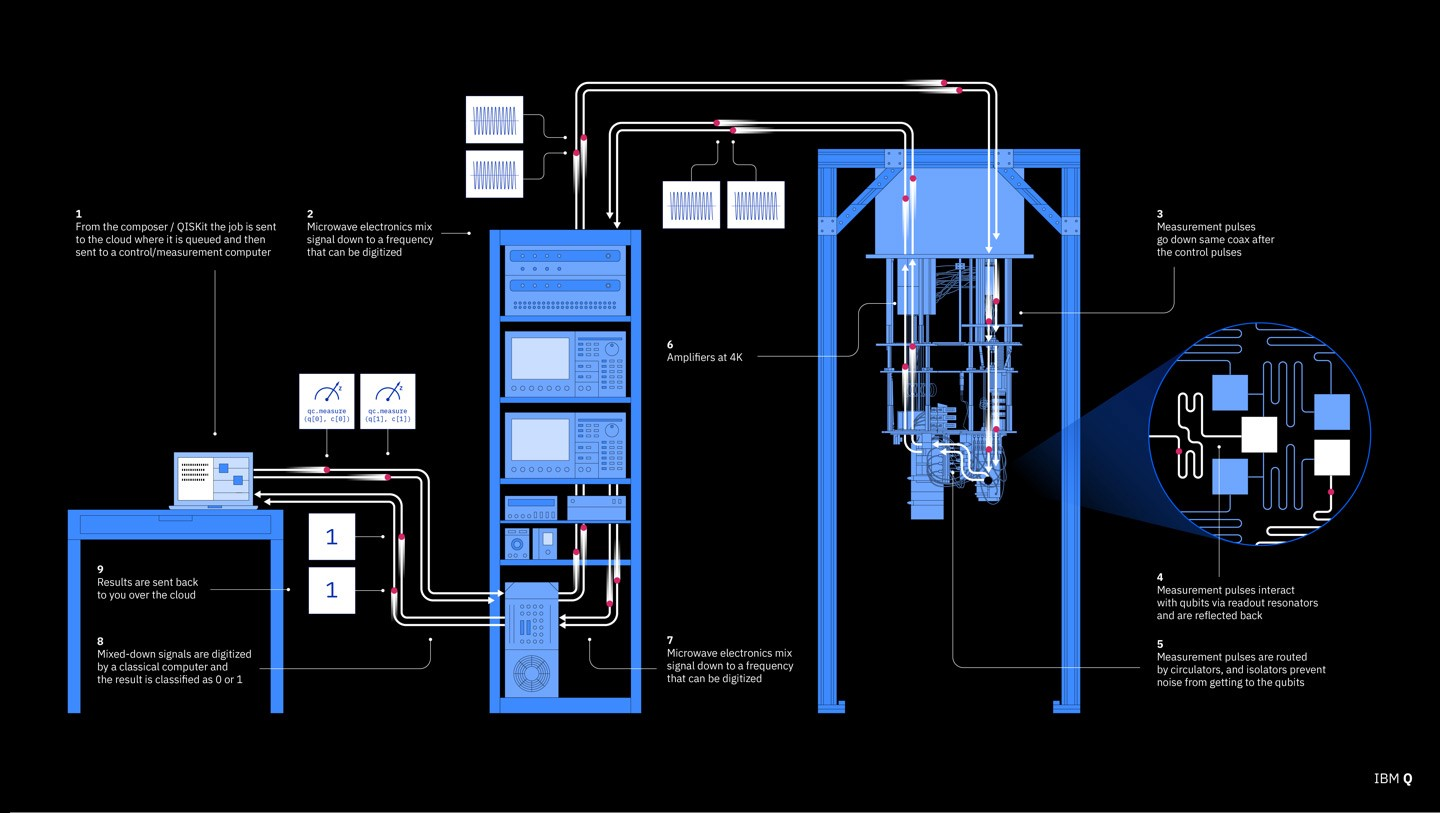
\includegraphics[width=\textwidth]{figures/quantum_computer.jpeg}
    \end{figure}

\end{frame}

\begin{frame}{Physical implementation}
\begin{multicols*}{2}
    \begin{figure}
        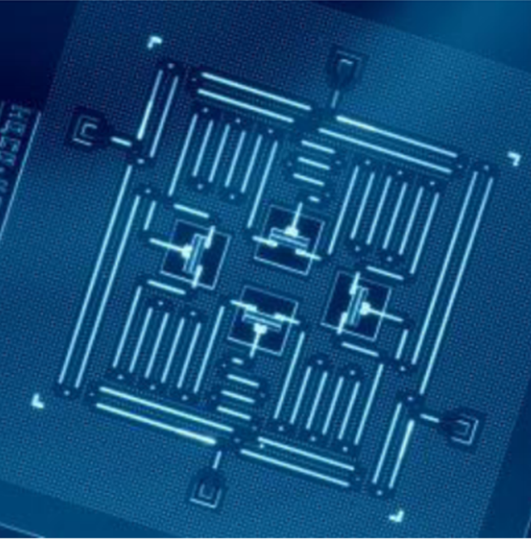
\includegraphics[width=0.30 \textwidth]{figures/superconducting_qubits.png}
        \caption{Superconducting device assembled by IBM}
        \end{figure}
        \begin{figure}
            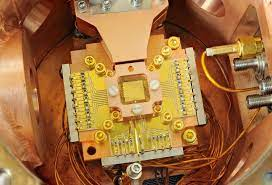
\includegraphics[width=0.30 \textwidth]{figures/ion_trap.jpeg}
            \caption{Chip based on trapped ions technology}
            \end{figure}
\end{multicols*}


\end{frame}

\begin{frame}{NISQ era}
    \begin{figure}
        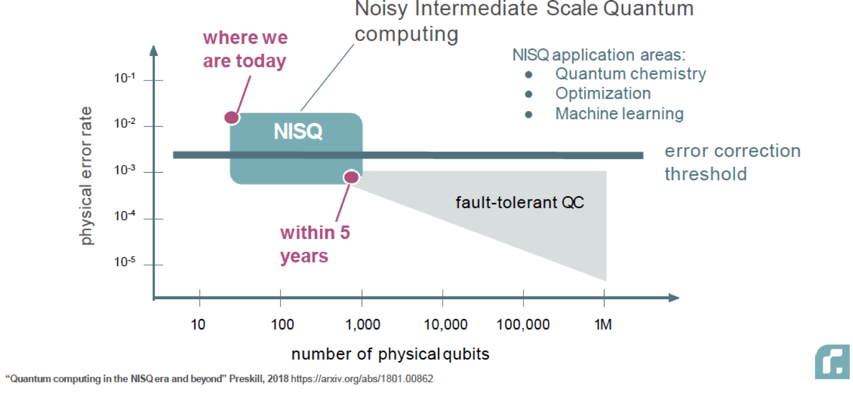
\includegraphics[width=\textwidth]{figures/nisq.png}
    \end{figure}
\end{frame}

\section{Languages for quantum computing}

    \begin{frame}{Challenge}
        \begin{figure}
            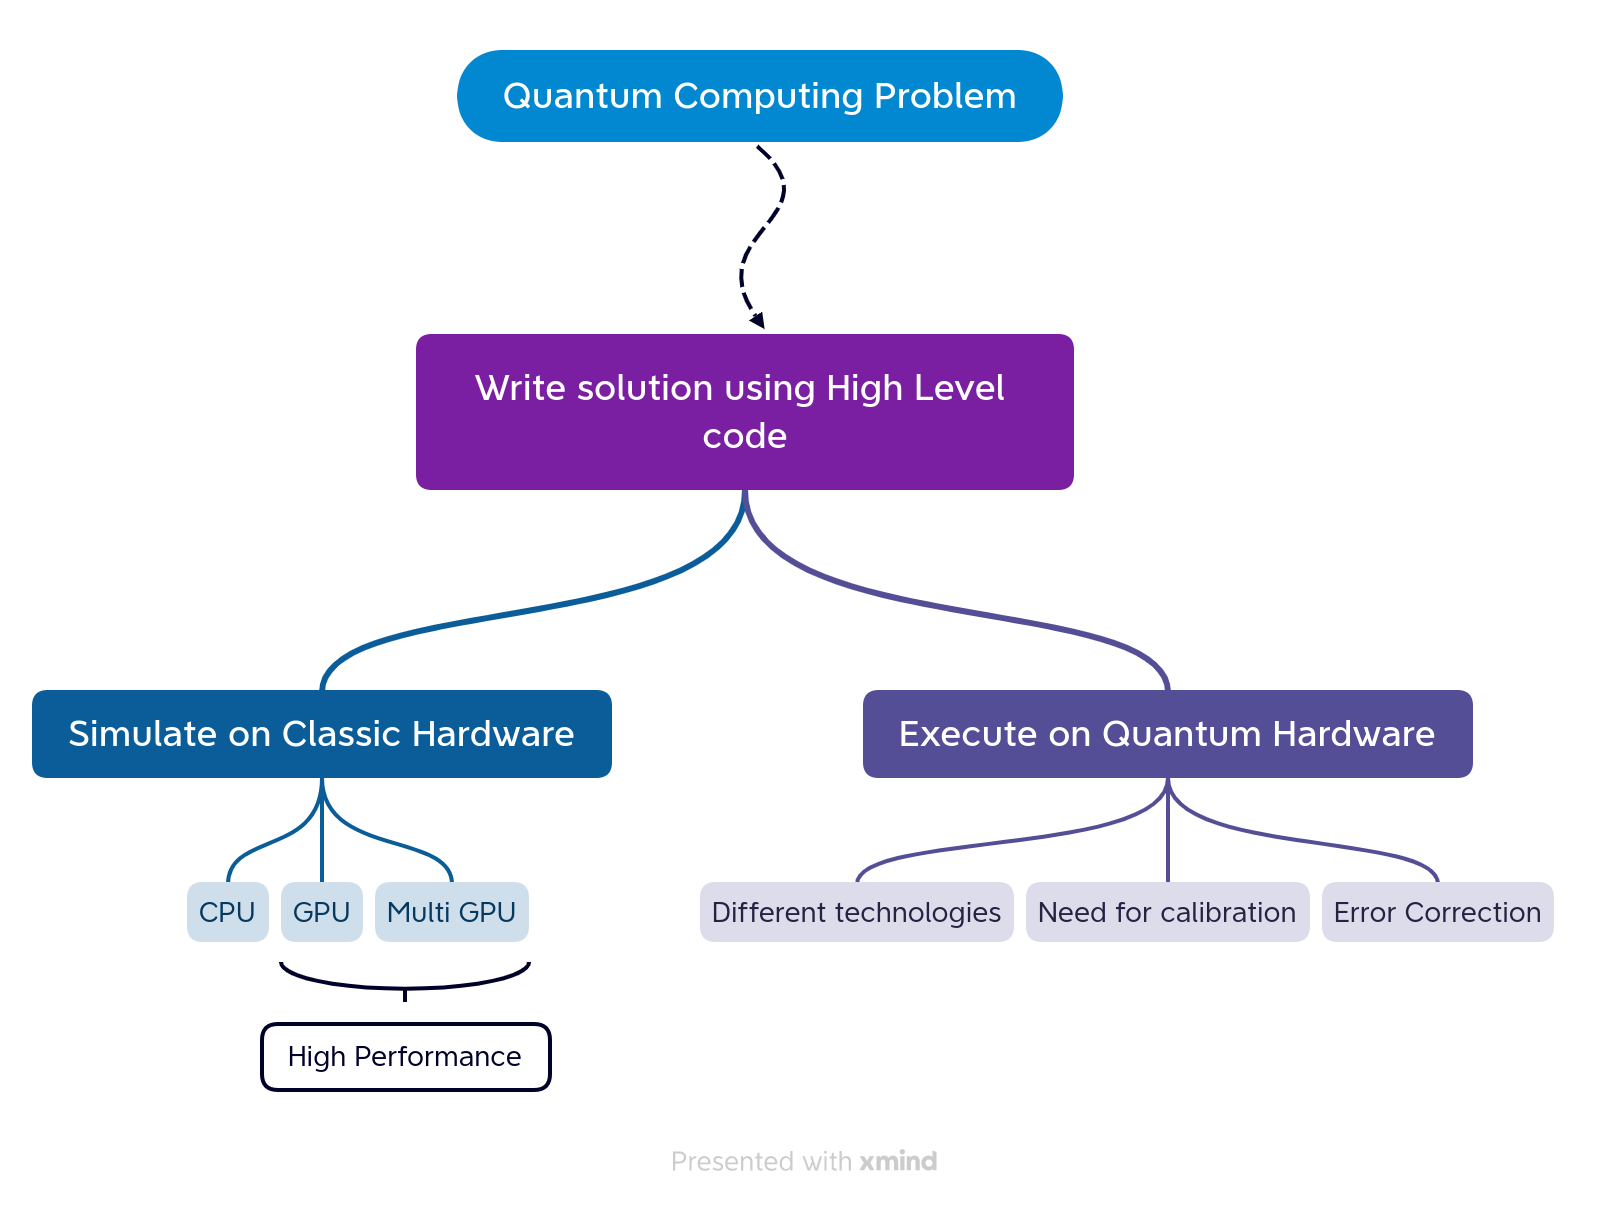
\includegraphics[width=\textwidth]{figures/intro.png}
        \end{figure}
        \centering
        \emph{Is to possible to create from scratch a framework for all of this?}
    \end{frame}


\begin{frame}{Introducing Qibo}
    Qibo is an \textbf{open-source} full stack API for quantum simulation and quantum hardware control and calibration.
    \begin{figure}
        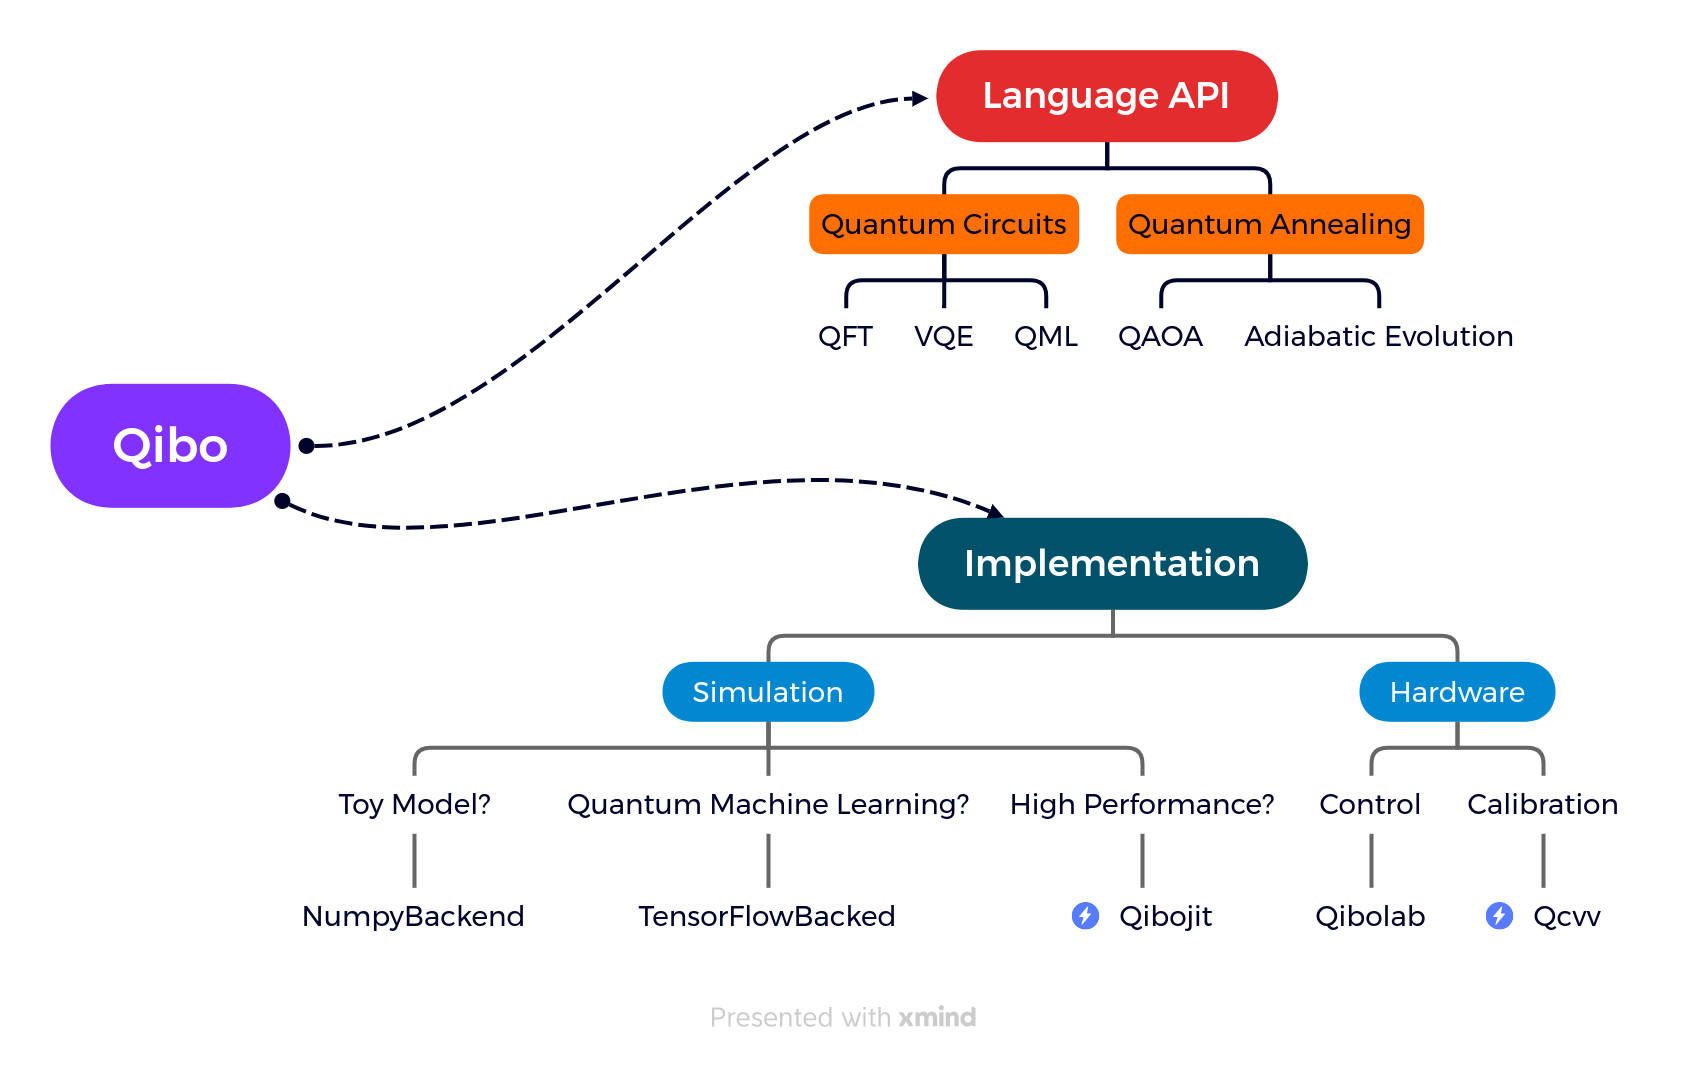
\includegraphics[width= \textwidth]{figures/Qibo.png}
    \end{figure}
\end{frame}

\section*{Thanks for listening!}

\end{document}